\begin{figure}[htbp]
    \centering
    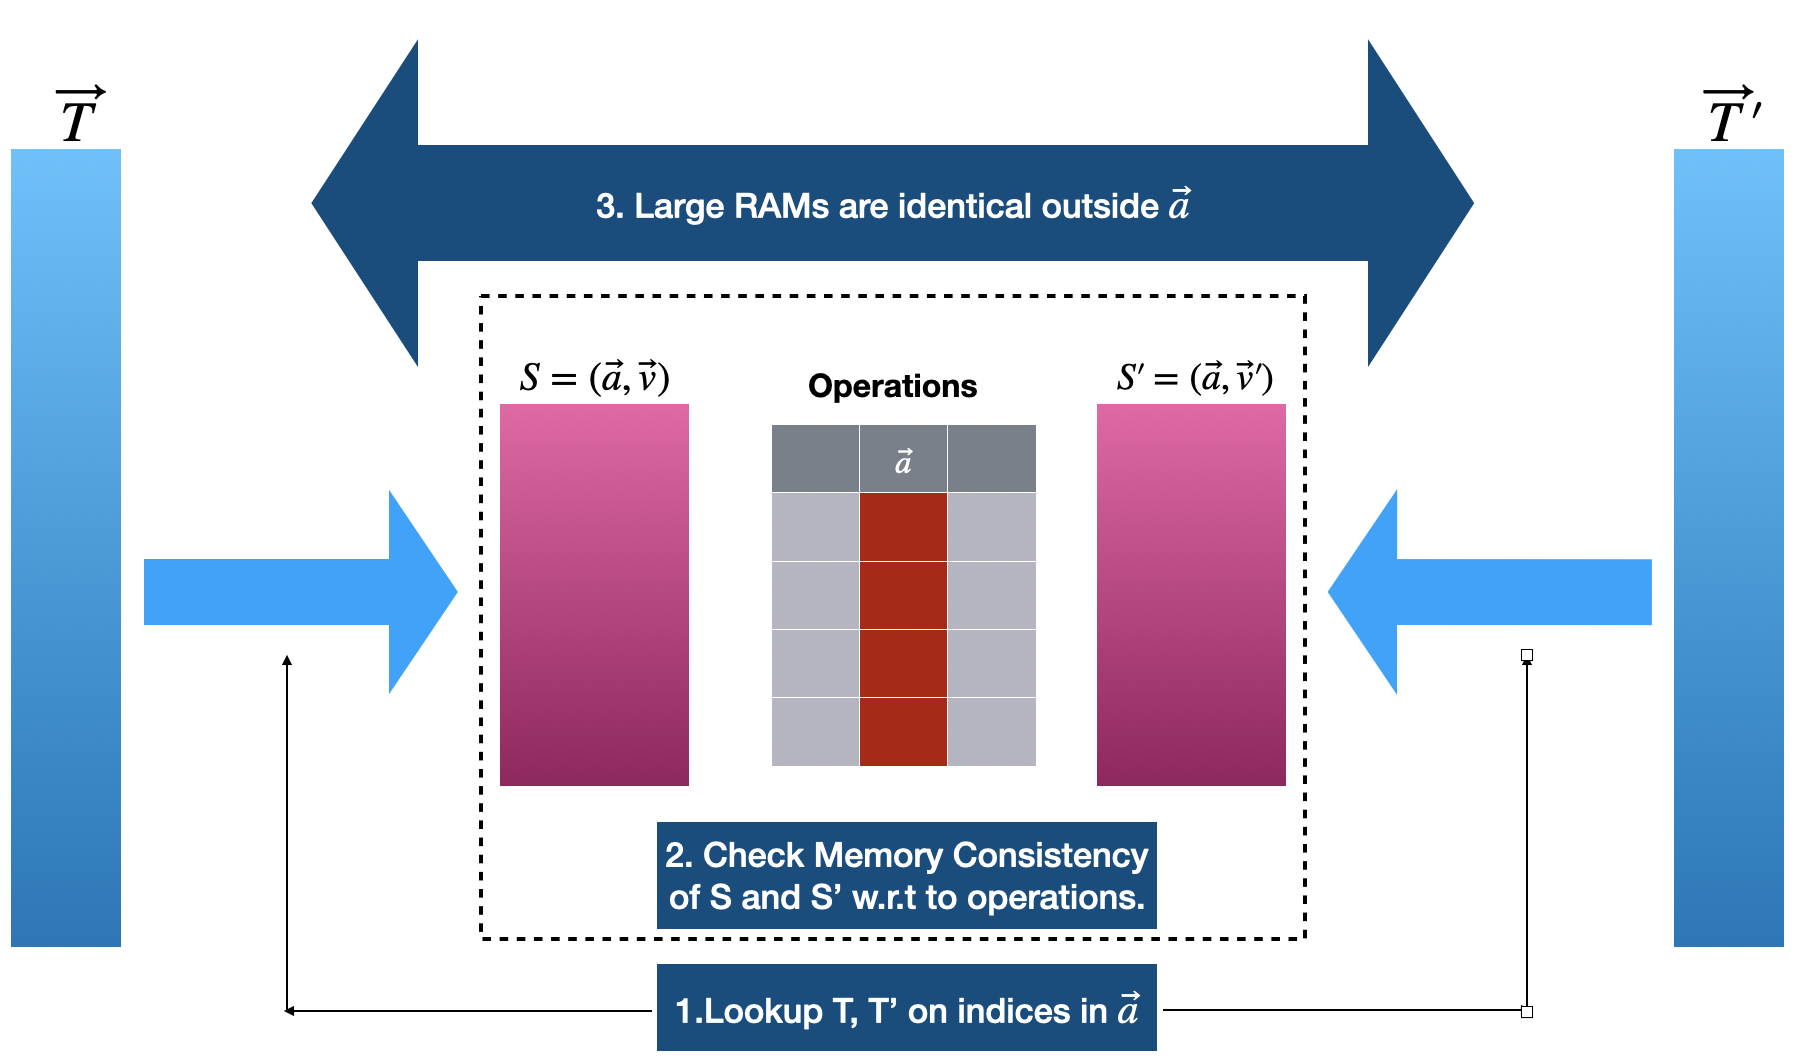
\includegraphics[width=\textwidth]{RAM-Lookup}
    \caption{Illustrating different steps of sub-linear lookup protocol between large RAMs $\vecT$ and $\vecT'$.}
    \label{fig:blueprint}
\end{figure}

The construction in the previous section results in prover complexity which is quasi-linear in both the
size of the RAM and the number of operations.
Our goal in this section is to achieve prover complexity which is {\em sublinear} in the size of the table. In
what follows, let $N$ denote the size of the RAM (upper-case to signify it's large) and $m$ denote the number
of operations in a batch. We will use a vectors in $\F^N$ to denote the ``large'' RAMs, where index column is implicitly
assumed to be $(1,\ldots,N)$.
Let $\vec{T},\vec{T'}\in \F^N$ denote the initial and final RAM states, and let $\vec{o}$ be
a sequence of $m$ operations which updates $\vec{T}$ to $\vec{T}'$. Let $\vec{a}\in \F^m$ denote the vector
of RAM indices referenced by the operations in $\vec{o}$, i.e $a_i$ is the index referenced by $i^{th}$ operation.
To prove the transformation of $\vec{T}$ to $\vec{T}'$ via operation sequence $\vec{o}$, we proceed as follows:
(i) We isolate sub-vectors $\vec{v}=(\vec{T}[a_1],\ldots,\vec{T}[a_m])$ and
$\vec{v}'=(\vec{T}'[a_1],\ldots,\vec{T}'[a_m])$ and use the committed index lookup protocol, described in
Section \ref{subsec:committed-index-lookup} to prove that vectors $\vec{v},\vec{v}'$ are correctly constructed,
(ii) We set $S=(\vec{a},\vec{v})$, $S'=(\vec{a},\vec{v}')$ and use the protocol of Section \ref{subsec:succ-args} to show
that $S'$ is the result of applying operations $\vec{o}$ on $S$, i.e. we show that the indices of the RAMs involved in the operation
are correctly updated, (iii) finally, we show that vectors $\vec{T}$ and $\vec{T}'$ are identical outside indices in $\vec{a}$.
We present polynomial protocol for the same in Section \ref{subsec:proximity-ram}. The aforementioned blueprint is illustrated
in Figure \ref{fig:blueprint}.

The efficiency of the above approach relies crucially on the efficiency of ``lookup argument'' in reducing the size of the RAMs for
linear time memory checking methods. Using recently developed lookup arguments directly is difficult, as thier efficiency relies on
table specific expensive pre-computation, which does not help when the table itself keeps changing. To circumvent this, we design a
lookup protocol, which efficiently proves lookup with access to ``approximate'' pre-computation. In particular, we call pre-computed
parameters for table $\vecT$ to be $\delta$-approximate with respect to table $\vecT'$ if the tables $\vecT$ and $\vecT'$ differ in
at most $\delta$ indices. Our protocol described in Section \ref{sec:update-protocol} allows proving lookup of $m$ indices with access
to a $\delta$-approximate setup in time $O(m^2+\delta\log^2 \delta)$. By optimally deferring $O(N\log N)$ pre-computation till we
accumulate $\delta \approx \sqrt{mN}$ updates, we achieve an amortized prover complexity of $O(m^2+\sqrt{mN})$.

Before proceeding, we introduce the subgroup $\setN=\{\xi,\ldots,\xi^N\}$ consisting of $N^{th}$ roots of unity,
over which we encode vectors in $\F^N$ as polynomials of degree less than $N$. Let $\{\mu_i(X)\}_{i=1}^N$ be the associated
lagrange basis polynomials over the set $\setN$. We also recall the set $\setV$ consisting of $m^{th}$ roots of unity
$\nu,\ldots,\nu^m$ with associated lagrange polynomials as $\{\tau_i(X)\}_{i=1}^m$. For $\vec{f}\in \F^N$, let
$\enc{f}{\setN}$ denote the polynomial encoding of $\vec{f}$ over $\setN$ given by $\sum_{i=1}^N f_i\mu_i(X)$. Similarly,
for $\vec{g}\in \F^m$, let $\enc{g}{\setV}$ denote its polynomial encoding over $\setV$ given by $\sum_{i=1}^m g_i\tau_i(X)$.


\subsection{Committed Index Lookup}\label{subsec:committed-index-lookup}
Let $m,N\in \N$ with $m < N$ and let $\srs$ denote a $\kzg$ setup over bilinear group $(\Gone,\Gtwo,\GT,\gone{1},\gtwo{1},e)$
large enough to commit to polynomials of degree $<N$. Prior works on lookup arguments (~\cite{CCS:ZBKMNS22,EPRINT:PosKat22} etc.)
have considered proving sub-vector relation over committed vectors, i.e, given commitments $c_t$ and $c_v$ to vectors $\vec{t}\in \F^N$
and $\vec{v}\in \F^m$, one proves that for all $i\in [m]$, there exists $j\in [N]$ such that $v_i=t_j$ .
We consider a slightly modified relation,
called {\em committed index lookup}  which also commits to indices where $\vec{v}$ appears in $\vec{t}$.

\begin{definition}\label{defn:comm-index-lookup}
We define the {\em committed index lookup} relation $\RLOOK$ to consist of tuples
$((c_t,c_a,c_v),(\vec{t},\vec{a},\vec{v}))$ where $c_t,c_a,c_v\in \Gone$, $\vec{t}\in \F^N$, $\vec{a},\vec{v}\in \F^m$ such
that $v_i = \vec{t}[a_i]=t_{a_i}$ for all $i\in [m]$ and $c_t = \kzgcommit(\srs, \enc{t}{\setN})$, $c_a=\kzgcommit(\srs,\enc{a}{\setV})$
and $c_v=\kzgcommit(\srs,\enc{v}{\setV})$.
\end{definition}

We present a polynomial protocol for the above relation, which is an adaptation of the lookup protocol from Caulk+ ~\cite{EPRINT:PosKat22}
to the indexed lookup case. Moreover, we do not aim for zero-knowledge. Let $T(X)=\enc{t}{\setN}$, $a(X)=\enc{a}{\setV}$ and
$v(X)=\enc{v}{\setV}$ denote the polynomials encoding the vectors $\vec{t},\vec{a}$ and $\vec{v}$ respectively. The prover commits
to these polynomials. Now $v_i = \vec{t}[a_i]$ for $i\in [m]$ is equivalent to $v(\nu^i) = T(\xi^{a(\nu^i)})$ for $i\in [m]$. To
obtain a polynomial protocol, the prover interpolates a polynomial $h(X)=\sum_{i=1}^m \xi^{a_i}\tau_i(X)$, which satisfies
$h(\nu^i)=\xi^{a(\nu^i)}$. To show that polynomial $h$ correctly ``exponentiates'' evaluations of $a(X)$, we consider the
polynomial $\ell(X)=\sum_{i=1}^N i\mu_i(X)$ which behaves like ``log'' over $\setN$ by evaluating to $i$ on $\xi^i$. Now, we see
that all constraints are encoded as polynomial identities below:
\begin{alignat}{3}
\ell(h(X)) &= a(X) &\quad \text{mod } Z_{\setV}(X) &&\quad\text{ encodes } &&\quad \forall i\in [m]:& h(\nu^i) = \xi^{a(\nu^i)}  \\
T(h(X)) &= v(X) &\quad \text{mod } Z_\setV(X) &&\quad\text{ encodes } &&\quad \forall i\in [m]:& v_i = \vec{t}[a_i] \\
Z_{\setN}(h(X)) &= 0 &\quad \text{mod } Z_\setV(X) &&\quad\text{ encodes } &&\quad \forall i \in [m]:& h(\nu^i)\in \setN
\end{alignat}
The above formulation involves composition with polynomials $\ell,T$ and $\vpolyN$ of degree $O(N)$, which is inefficient. We use the trick from
\cite{EPRINT:PosKat22}, where we work with low-degree restrictions of polynomials such as $T, \ell$ over the set
$\setN_I=\{{h(\nu^i)}: i\in I\}=\{\xi^{a_i}:i\in I\}\subseteq \setN$, where $I=\{a_i: i\in [m]\}$. To this end, the prover
commits to the polynomial $Z_I(X)=\prod_{i\in I}(X-\xi^i)$, and low degree ($<m$) restrictions $T_I, \ell_I$ of $T$ and $\ell$
on $\setN_I$ respectively. The polynomial protocol then checks the following:
\begin{alignat}{2}\label{eq:poly-comm-index}
T(X) - T_I(X) &= 0 &\quad \text{ mod } Z_I(X) &&,\quad T_I(h(X)) &= v(X) &\quad \text{ mod } Z_{\setV}(X) \\
\ell(X) - \ell_I(X) &= 0 &\quad \text{ mod } Z_I(X) &&,\quad \ell_I(h(X)) &= a(X) &\quad \text{ mod } Z_{\setV}(X) \\
Z_{\setN}(X) &= 0 &\quad \text{ mod } Z_I(X) &&,\quad Z_I(h(X)) &= 0 &\quad \text{ mod } Z_{\setV}(X)
\end{alignat}
While the identities on the left still involve a degree $N$ polynomial, we can use the $\srs$ to check the polynomial
identity at the point $\tau$ encoded in the $\srs$. For example, we can evaluate the encoded quotient $\gtwo{Q(X)} =$
$\gtwo{\frac{(T(X) - T_I(X)}{Z_I(X)}}$ using the relation:
\begin{equation*}
\gtwo{\frac{T(X)-T_I(X)}{Z_I(X)}} = \sum_{i\in I}\frac{1}{Z_I'(\xi^i)}\gtwo{\frac{T(X)-t_i}{X-\xi^i}}
\end{equation*}
By pre-computing the $\kzg$ proofs $W_1^i=\gtwo{\frac{T(X)-t_i}{X-\xi^i}}$ for all $i\in [N]$, the encoded quotient can be
evaluated using $O(m)$ $\Gtwo$-operations and $O(m\log^2 m)$ $\F$-operations. The identity is then checked using a real
pairing check $e(\gone{T(X)}-\gone{T_I(X)},\gtwo{1})=e(\gone{Z_I(X)},\gtwo{Q(X)})$.
Similarly, we also pre-compute the encoded
quotients $W_2^i=\gtwo{\frac{\ell(X) - i}{X-\xi^i}}$ and $W_3^i=\gtwo{\frac{\vpolyN(X)}{X-\xi^i}}$ for all $i\in [N]$.
The quotients can be computed in time $O(N\log N)$ using the techniques in ~\cite{EPRINT:FeiKho23}.
The polynomial relations over $Z_\setV$ can be checked in a standard manner via evaluations at a random point with $O(m^2)$ prover effort.
Thus, we have:
\begin{lemma}\label{lem:comm-index-lookup}
Assuming $\kzg$ is extractable polynomial commitment scheme, there exists a succinct argument of knowledge for
the relation $\RLOOK$ with prover complexity of $O(m^2)$, given access to pre-computed parameters of size $O(N)$.
\end{lemma}

\subsection{Proximity of RAM States}\label{subsec:proximity-ram}
For a vector $\vec{a}\in [N]^m$, let $\uniq{a}=\{a_i: i\in [m]\}$ denote the subset of unique values in $\vec{a}$. We call two
RAM states $\vecT, \vecT'\in \F^N$ to be $\vec{a}$-{\em identical} if $\vecT[i]=\vecT'[i]$ for all $i\not\in\uniq{a}$. As before,
let $T(X),T'(X)$ and $a(X)$ be polynomials encoding the vectors $\vecT,\vecT'$ (over $\setN$) and $\vec{a}$ (over $\setV$). The
polynomial protocol involves proving the relation $Z_I(X)(T(X) - T'(X)) = 0$ over $Z_\setN$ where $Z_I(X)=\prod_{i\in I}(X-\xi^i)$
for $I=\uniq{a}$ denotes the vanishing polynomial over the support of $\vec{a}$.
The prover commits to polynomial $Z_I$ and proves (i) $Z_I(T - T') = 0 \text{ mod } Z_\setH$ and (ii) $Z_I$ is the vanishing
polynomial of the support of vector $\vec{a}$. To prove the first relation, the prover computes the polynomial $Q(X)$ as below:
\begin{align}\label{eq:poly-q}
Q(X) &= \frac{(T(X)-T'(X))\cdot Z_I(X)}{Z_\setN(X)} \nonumber \\
&= \sum_{i\in I}\frac{(t_i - t_i')\mu_i(X)}{Z_\setN(X)} Z_I(X) \nonumber \\
\intertext{ Substituting, $\Delta_i=t_i-t_i'$, $\mu_i(X)=\vpolyN(X)/(\vpolyN'(\xi^i)(X-\xi^i))$ }
&=\sum_{i\in I}\frac{\Delta_i}{Z_\setN'(\xi^i)}\left(\frac{Z_I(X)}{X-\xi^i}\right) = \sum_{i\in I}\frac{\Delta_i Z_I'(\xi^i)}{Z_\setN'(\xi^i)}\kappa_i(X)
\end{align}
In the above, the summation only runs over indices in $I$, as $t_i=t_i'$ for $i\not\in I$. In the final equality, we use
$\kappi_i(X) = Z_I(X)/(Z_I'(\xi^i)(X-\xi^i))$ for $i\in I$ which we recognize as the lagrange basis polynomials for the set
$\{\xi^i: i\in I\}$. Thus, Equation \eqref{eq:poly-q} implies that $Q$ is a degree $|I|-1$ polynomial, with
$Q(\xi^i)=\Delta_i Z_I'(\xi^i)/\vpolyN'(\xi^i)$ for $i\in I$. The prover can therefore interpolate $Q(X)$ (in power basis)
in $O(|I|\log^2 |I|)$ $\F$-operations and compute $\gtwo{Q(X)}$ in $O(|I|)$ $\Gtwo$-operations.

Next, the prover needs to show that $Z_I(X)$ is indeed the vanishing polynomial of $\setN_I=\{\xi^i: i\in I\}$ where $I=\uniq{a}$.
We again use the polynomial $h(X)=\sum_{i=1}^m \xi^{a_i}\tau_i(X)$ which interpolates the vector $(\xi^{a_1},\ldots,\xi^{a_m})$.
The correctness of the $h$ polynomial can be established using the restriction $\ell_I$ of ``log'' polynomial $\ell$ as before.
We show that $Z_I(h(X)) = 0$ over $Z_\setV$ which shows that $Z_I$ vanishes over entire vector interpolated
by $h$. To assert that $Z_I$ has no additional roots, the prover commits to the product polynomial
$K(X)=\prod_{i=1}^m (X - h(\nu^i))$ and the quotient polynomial $q(X)=K(X)/Z_I(X)$. The verifier checks the polynomial identities
at $\alpha$, i.e $K(\alpha)=q(\alpha)Z_I(\alpha)$ and $K(\alpha)=\prod_{i=1}^m(\alpha - h(\nu^i))$. The former is easily accomplished
using evaluation proofs for $K,q$ and $Z_I$ at $\alpha$. For checking the latter, the prover commits to another polynomial
$u(X)$ satisfying $u(\nu^i)=\prod_{j=1}^{i-1}\big((\alpha - h(\nu^j))/(1 + \beta\tau_1(\nu^j))\big)$ for $i\in [m]$
where $\beta=K(\alpha) - 1$.
The verifier ensures the correctness of $u(X)$ by checking:
\begin{align*}
\tau_1(X)(u(X) - 1) &= 0 \text{ mod } Z_{\setV} \\
u(\nu X)(1+\beta \tau_1(X))-u(X)(\alpha - h(X)) &= 0 \text{ mod } Z_\setV.
\end{align*}
Note that the constraints on $u(X)$ essentially
ensure that $K(\alpha)\cdot 1\cdots 1 = (\alpha - h(\nu))\cdots (\alpha - h(\nu^m))$, which follows from the fact that
$u(\nu)=u(\nu^{m+1})=1$.

\subsection{Batching Efficient RAM: Combined Protocol}\label{subsec:all-together}
We put the entire protocol together now. Let $\setind$ denote the set of indices $\{1,\ldots,N\}$, and $\mathcal{I}_N$
denote the vector $(1,\ldots,N)$. We formally define the committed RAM relation for which we present the argument of
knowledge in this section.
\begin{definition}\label{defn:committed-ram}
We define the {\em committed ram} relation
$\CRAM$ to consist of tuples $((c_T, c_T', c_\op, c_a, c_w),(\vecT, \vecT',\vec{\op},\vec{a},\vec{w}))$
such that:
\begin{itemize}[leftmargin=1em]
\item $(T,\vec{o},T')\in \LRAM{I}{N}{m}$ for $T=(\setind_N,\vecT)$, $T'=(\setind_N,\vecT')$ and $\vec{o}=(o_1,\ldots,o_m)$
where $o_i=(\op_i, a_i, w_i)\in \RAMOp{I}$ for all $i\in [m]$.
\item $c_T=\kzgcommit(\srs,\enc{T}{\setN})$, $c_T'=\kzgcommit(\srs,\enc{T'}{\setN})$, $c_\op=\kzgcommit(\srs,\enc{\op}{\setV})$,
$c_a=\kzgcommit(\srs,\enc{a}{\setV})$ and $c_w$ $=$ \\ $\kzgcommit(\srs,\enc{w}{\setV})$.
\end{itemize}
\end{definition}
As outlined in the blueprint, the prover first commits to ``smaller'' RAMs $S=(\vec{a},\vec{v})$ and $S'=(\vec{a},\vec{v}')$
where $\vec{v}=\vecT[\vec{a}]$ and $\vec{v}'=\vecT'[\vec{a}]$. The prover commits to $S$ and $S'$ by sending commitments
$c_v$ and $c_v'$ to $\vec{v}$ and $\vec{v}'$. Then the prover and verifier execute the committed index lookup protocol to
prove:
\begin{equation}
(c_T, c_a, c_v)\in \RLOOK\, \wedge\, (c_T', c_a, c_v')\in \RLOOK
\end{equation}
The verifier uses a random challenge $\chi\gets \F$ to reduce two instances of $\RLOOK$ to one instance
$(c_T + \chi c_T', c_a, c_v + \chi c_v')\in \RLOOK$. Thereafter, the prover and verifier execute the argument for
showing $(S,\vec{o},S')\in \LRAM{I}{m}{m}$ as described in Section \ref{subsec:succ-args}. Finally, we show that
RAMs $\vecT$ and $\vecT'$ are $\vec{a}$-identical using the protocol in Section \ref{subsec:proximity-ram}.

\section{Fast Lookups from Approximate Pre-Processing}\label{sec:update-protocol}












